\documentclass[12pt,a4paper]{article}
\usepackage[UTF8]{ctex}
\usepackage{float}
\usepackage{amsmath}
\usepackage{enumerate}
\usepackage{booktabs}
\usepackage{graphicx}
\usepackage{longtable}
\usepackage{subfigure}
\usepackage{amsfonts}

\usepackage{url}

% for plotting 
\usepackage{caption}
\usepackage{pgfplots}

% for pseudo code 
\usepackage{algorithm}
\usepackage[noend]{algpseudocode}

% for reference 
\usepackage{hyperref}
\usepackage{cleveref}
\crefname{equation}{方程}{方程}
\Crefname{equation}{方程}{方程}
\crefname{table}{表}{表}
\Crefname{table}{表}{表}
\crefname{figure}{图}{图}
\Crefname{figure}{图}{图}

% for code 
\usepackage{listings}
\usepackage{xcolor}
\usepackage{inconsolata}
\definecolor{darkgreen}{rgb}{0,0.6,0}

\lstset {
    basicstyle=\footnotesize\ttfamily, % basic font setting
    breaklines=true, 
    frame=single,     % {single, shadowbox, bottomline}
    keywordstyle=\color{blue}, 
    commentstyle=\color{darkgreen},
    stringstyle=\color{red},
    showstringspaces=false,
    % backgroundcolor=\color{black!5}, % set backgroundcolor
    % numbers=left, 
    % numberstyle=\consolas,
}

% Microsoft Word A4 paper default layout 
\usepackage[a4paper, left=3.18cm, right=3.18cm, top=2.54cm, bottom=2.54cm]{geometry}

\captionsetup[figure]{name={图}}
\captionsetup[table]{name={表}}

\title{DIP Lab 4: Image Compression}
\author{2017011620 \quad 计73 \quad 李家昊}
\date{\today}

\begin{document}

\maketitle

\section{实验一}

\subsection{实验原理}

本实验将实现离散余弦变换(DCT)及其逆变换(IDCT),其中DCT将信号从时域映射到频域,而IDCT将信号从频域映射到时域。

对于一维DCT,给定一个$N$维向量$\mathbf{x}$,其$N$点DCT为$\mathbf{y}$,则有,
\begin{equation}
    y_k = \alpha_k^{(N)} \sum_{n=0}^{N-1} x_n \cos\left(\frac{(2n+1)k\pi}{2N}\right), \quad k = 0,1,2,\cdots,N-1
\end{equation}

其中,
\begin{equation}
    \alpha_k^{(N)} = \begin{cases}
        \sqrt{1/N}, & k = 0 \\
        \sqrt{2/N}, & k \ge 1 \\
    \end{cases}
\end{equation}

记矩阵$\mathbf{A}_N = (a_{kn}^{(N)}) \in \mathbb{R}^{N \times N}$,其中,
\begin{equation}
    a_{kn}^{(N)} = \alpha_k^{(N)} \cos\left(\frac{(2n+1)k\pi}{2N}\right), \quad k,n = 0,1,2,\cdots,N-1
\end{equation}

则一维DCT可以表示成矩阵形式,直接计算的时间复杂度为$O(N^2)$,
\begin{equation}
    \mathbf{y} = \mathbf{A}_N \mathbf{x}
\end{equation}

对于二维DCT,给定一个$M\times N$矩阵$\mathbf{X}$,其二维DCT为$\mathbf{Y}$,则有,
\begin{equation}\label{eq:dct2d}
    Y_{uv} = \alpha_u^{(M)}\alpha_v^{(N)} \sum_{x=0}^{M-1} \sum_{y=0}^{N-1} X_{xy} \cos \left(\frac{(2x+1)u\pi}{2M}\right) \cos\left(\frac{(2y+1)v\pi}{2N}\right)
\end{equation}

将\Cref{eq:dct2d}稍作变换可知,二维DCT可以看作两次一维DCT,
\begin{equation}\label{eq:dct1d1d}
    Y_{uv} = \alpha_v^{(N)} \sum_{y=0}^{N-1}\left\{\cos\left(\frac{(2y+1)v\pi}{2N}\right) \left[ \alpha_u^{(M)} \sum_{x=0}^{M-1} X_{xy} \cos \left(\frac{(2x+1)u\pi}{2M}\right) \right] \right\}
\end{equation}

同样有$\mathbf{A}_M = (a_{ux}^{(M)}) \in \mathbb{R}^{M\times M}$,$\mathbf{A}_N = (a_{vy}^{(N)}) \in \mathbb{R}^{N\times N}$,根据\Cref{eq:dct1d1d},首先对每一列做一维DCT,即$\mathbf{A}_M \mathbf{X}$,再对每一行做一维DCT,即$(\mathbf{A}_N(\mathbf{A}_M \mathbf{X})^T)^T$,这样就得到了二维DCT的矩阵形式,计算的时间复杂度为$O(MN(M+N))$,
\begin{equation}
    \mathbf{Y} = \mathbf{A}_M \mathbf{X} \mathbf{A}_N^T
\end{equation}

容易验证$\mathbf{A}_N$为正交矩阵,由此可得一维和二维IDCT分别为,
\begin{equation}
    \mathbf{x} = \mathbf{A}_N^T \mathbf{y}, \quad \mathbf{X} = \mathbf{A}_M^T \mathbf{Y} \mathbf{X}_N
\end{equation}

\subsection{实验结果及分析}

首先选取一个$8\times 8$区域作为例子,如\Cref{fig:block_pos},对该区域分别进行二维DCT和两次一维DCT,频域图像和恢复的图像如\Cref{fig:block_dct}。经过计算,两种DCT方式处理的图片经过IDCT还原后,信噪比均为$+\infty$,说明两种处理方式是等价的,这也与实验原理部分的理论分析相符。

\begin{figure}[H]
    \centering
    \subfigure[帽檐处白框内的$8\times 8$区域]{
        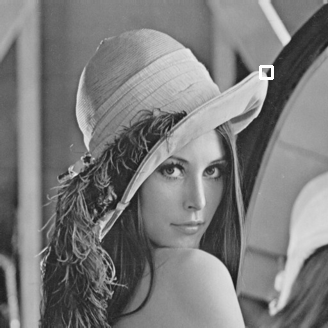
\includegraphics[width=0.3\textwidth]{../output/block_pos.png}
    }
    \subfigure[放大的$8\times 8$区域]{
        
\includegraphics[width=0.3\textwidth,interpolate=false]{../output/block.png}
    }
    \caption{选取女生帽檐处白框内的$8\times 8$区域}
    \label{fig:block_pos}
\end{figure}

\begin{figure}[H]
    \centering
    \subfigure[DCT2D]{
        
\includegraphics[width=0.22\textwidth]{../output/block_dct2d.png}
    }
    \subfigure[DCT2D-IDCT]{
        
\includegraphics[width=0.22\textwidth,interpolate=false]{../output/block_dct2d_idct.png}
    }
    \subfigure[DCT1Dx2]{
        
\includegraphics[width=0.22\textwidth]{../output/block_dct1d1d.png}
    }
    \subfigure[DCT1Dx2-IDCT]{
        
\includegraphics[width=0.22\textwidth,interpolate=false]{../output/block_dct1d1d_idct.png}
    }
    \caption{在$8\times 8$区域内二维DCT和两次一维DCT的对比结果}
    \label{fig:block_dct}
\end{figure}

接下来将原图分割为若干个$8\times 8$区域,每个区域内分别用二维DCT和两次一维DCT处理,得到频域图像后,仅保留左上角低频部分的系数,去掉高频部分,在不同的保留比例下,得到的结果如\Cref{fig:keep_rate},对应的峰值信噪比(PSNR)如\Cref{tab:keep_rate_psnr}。实验结果又一次验证了,二维DCT和两次一维DCT的处理效果是完全相同的。同时也可以看出,图像的大部分信息主要集中在低频部分,当保留比例为$1/64$时,得到的结果依然是可辨认的,如\Cref{fig:keep_rate_64}。

\begin{figure}[H]
    \centering
    \subfigure[保留所有系数]{
        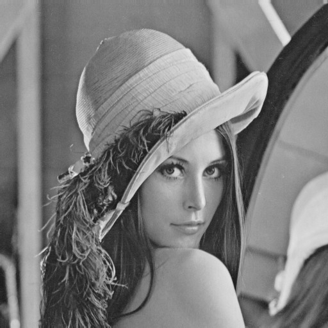
\includegraphics[width=0.22\textwidth]{../output/dst_8_8.png}
    }
    \subfigure[保留1/4系数]{
        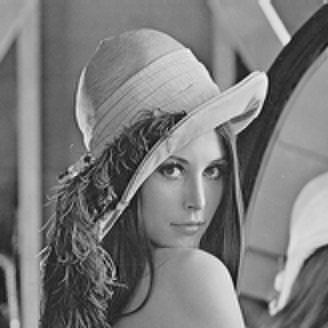
\includegraphics[width=0.22\textwidth]{../output/dst_8_4.png}
    }
    \subfigure[保留1/16系数]{
        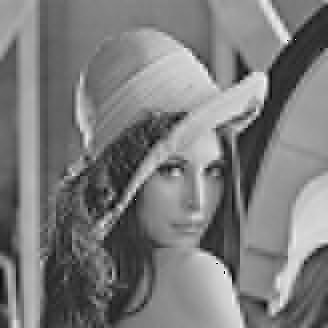
\includegraphics[width=0.22\textwidth]{../output/dst_8_2.png}
    }
    \subfigure[保留1/64系数]{
        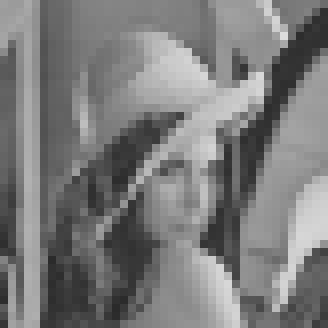
\includegraphics[width=0.22\textwidth]{../output/dst_8_1.png}
        \label{fig:keep_rate_64}
    }
    \caption{保留不同比例的频域系数的对比结果}
    \label{fig:keep_rate}
\end{figure}

\begin{table}[H]
    \centering
    \caption{在不同的系数保留比例下,复原图像的峰值信噪比PSNR}
    \label{tab:keep_rate_psnr}
    \begin{tabular}{c|cccc}
        \toprule
        Method $\backslash$ \#Coef. & 1/1 & 1/4 & 1/16 & 1/64\tabularnewline
        \midrule
        DCT2D & 67.39 & 32.95 & 26.41 & 22.04\tabularnewline
        DCT1Dx2 & 67.39 & 32.95 & 26.41 & 22.04\tabularnewline
        \bottomrule
    \end{tabular}
\end{table}

调整方块区域的大小,再次进行实验,实验结果如\Cref{tab:block_psnr}。可以看出,方块区域越大,保留比例越低,那么丢失的信息就越多,block effect就越明显,PSNR也就越低。

\begin{table}[H]
    \centering
    \caption{在不同的方块大小以及系数保留比例下,复原图像的峰值信噪比PSNR}
    \label{tab:block_psnr}
    \begin{tabular}{c|cccccc}
        \toprule
        Block $\backslash$ \#Coef. & 1/1 & 1/4 & 1/16 & 1/64 & 1/256 & 1/1024\tabularnewline
        \midrule
        \(1\times 1\) & $+\infty$ & & & & &\tabularnewline
        \(2\times 2\) & 74.23 & 29.95 & & & &\tabularnewline
        \(4\times 4\) & 70.58 & 31.62 & 25.35 & & &\tabularnewline
        \(8\times 8\) & 67.39 & 32.95 & 26.41 & 22.04 & &\tabularnewline
        \(16\times 16\) & 62.60 & 33.64 & 27.33 & 22.93 & 19.36 &\tabularnewline
        \(32\times 32\) & 60.61 & 33.93 & 27.69 & 23.51 & 20.09 &
        17.15\tabularnewline
        \bottomrule
    \end{tabular}
\end{table}

\section{实验二}

\subsection{实验原理}

实验一通过直接去掉某些高频系数来压缩图像,这往往会带来一些block effect。为了缓解这一问题,实验二引入了量化表来过滤高频,这也是JPEG压缩格式的做法。在一个$8\times 8$方块内,记量化表为$Q$,原始图像通过DCT得到频谱为$\mathbf{Y}$,则量化后的结果为,
\begin{equation}
    Y_q(u,v) = \text{round}\left(\frac{Y(u,v)}{Q(u,v)}\right)
\end{equation}

量化完成后,再通过编码,就生成了压缩后的图像数据。

恢复图像时,首先解码,然后反量化,
\begin{equation}
    Y(u,v) = Y_q(u,v) \cdot Q(u,v)
\end{equation}

再进行IDCT,就可以恢复图像了。

量化表有很多种设计,本次实验主要对比三种量化表,分别是Canon DIGITAL IXUS 60 (fine),记为$Q_1$,
\begin{equation}
    Q_1 = \left(\begin{matrix}
        1 & 1 & 1 & 2 & 3 & 6 & 8 & 10 \\
        1 & 1 & 2 & 3 & 4 & 8 & 9 & 8 \\
        2 & 2 & 2 & 3 & 6 & 8 & 10 & 8 \\
        2 & 2 & 3 & 4 & 7 & 12 & 11 & 9 \\
        3 & 3 & 8 & 11 & 10 & 16 & 15 & 11 \\
        3 & 5 & 8 & 10 & 12 & 15 & 16 & 13 \\
        7 & 10 & 11 & 12 & 15 & 17 & 17 & 14 \\
        14 & 13 & 13 & 15 & 15 & 14 & 14 & 14
    \end{matrix}\right)
\end{equation}

Nikon CoolPix L12 (fine),记为$Q_2$,
\begin{equation}
    Q_2 = \left(\begin{matrix}
        2 & 1 & 1 & 2 & 3 & 5 & 6 & 7 \\
        1 & 1 & 2 & 2 & 3 & 7 & 7 & 7 \\
        2 & 2 & 2 & 3 & 5 & 7 & 8 & 7 \\
        2 & 2 & 3 & 3 & 6 & 10 & 10 & 7 \\
        2 & 3 & 4 & 7 & 8 & 13 & 12 & 9 \\
        3 & 4 & 7 & 8 & 10 & 12 & 14 & 11 \\
        6 & 8 & 9 & 10 & 12 & 15 & 14 & 12 \\
        9 & 11 & 11 & 12 & 13 & 12 & 12 & 12
    \end{matrix}\right)
\end{equation}

以及Jpeg Standard,记为$Q_3$,
\begin{equation}
    Q_3 = \left(\begin{matrix}
        16 & 11 & 10 & 16 & 24 & 40 & 51 & 61 \\
        12 & 12 & 14 & 19 & 26 & 58 & 60 & 55 \\
        14 & 13 & 16 & 24 & 40 & 57 & 69 & 56 \\
        14 & 17 & 22 & 29 & 51 & 87 & 80 & 62 \\
        18 & 22 & 37 & 56 & 68 & 109 & 103 & 77 \\
        24 & 35 & 55 & 64 & 81 & 104 & 113 & 92 \\
        49 & 64 & 78 & 87 & 103 & 121 & 120 & 101 \\
        72 & 92 & 95 & 98 & 112 & 100 & 103 & 99
    \end{matrix}\right)
\end{equation}

\subsection{实验结果及分析}

三种量化表处理后,复原图像如\Cref{fig:quant_table},峰值信噪比如\Cref{tab:quant_table_psnr}。三张复原图像中,肉眼几乎看不出区别,从PSNR数值来看,Canon和Nikon差异不大,但两者均显著优于JPEG。原因可能是JPEG量化表的数值更大,压缩比更高,带来的数据流失也相对更多。

\begin{figure}[H]
    \centering
    \subfigure[Canon]{
        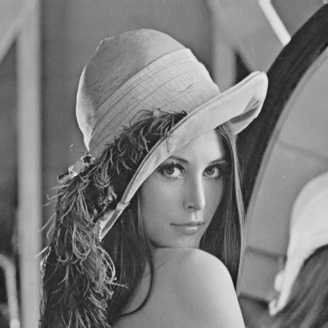
\includegraphics[width=0.3\textwidth]{../output/quant_canon.png}
    }
    \subfigure[Nikon]{
        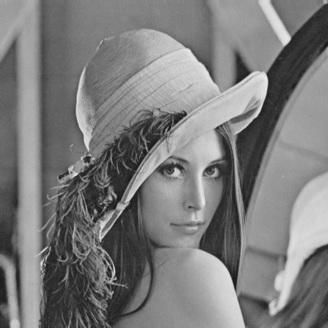
\includegraphics[width=0.3\textwidth]{../output/quant_nikon.png}
    }
    \subfigure[JPEG]{
        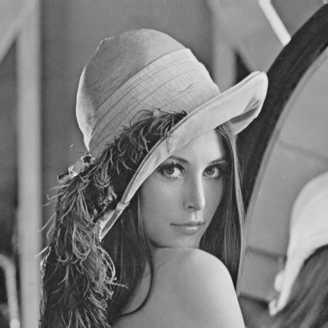
\includegraphics[width=0.3\textwidth]{../output/quant_jpeg.png}
    }
    \caption{三种量化表的处理结果}
    \label{fig:quant_table}
\end{figure}

\begin{table}[H]
    \centering
    \caption{三种量化表处理后,复原图像的峰值信噪比PSNR}
    \label{tab:quant_table_psnr}
    \begin{tabular}{c|ccc}
        \toprule
        & Canon & Nikon & JPEG\tabularnewline
        \midrule
        PSNR & 42.93 & 43.85 & 35.15\tabularnewline
        \bottomrule
    \end{tabular}
\end{table}

进一步考虑在量化表前添加一个系数$a$,以$aQ$来作量化处理,随着$a$的变化,PSNR的变化如\Cref{fig:quant_factor_psnr},压缩率变化如\Cref{fig:quant_factor_compress}。可以看到,随着$a$的增长,量化表的数值越大,图像压缩率越高,损失的信息越多,因此PSNR越低。压缩比和PSNR通常是矛盾的,在实际应用中,需要找到两者之间的平衡。

\begin{figure}[H]
    \centering
    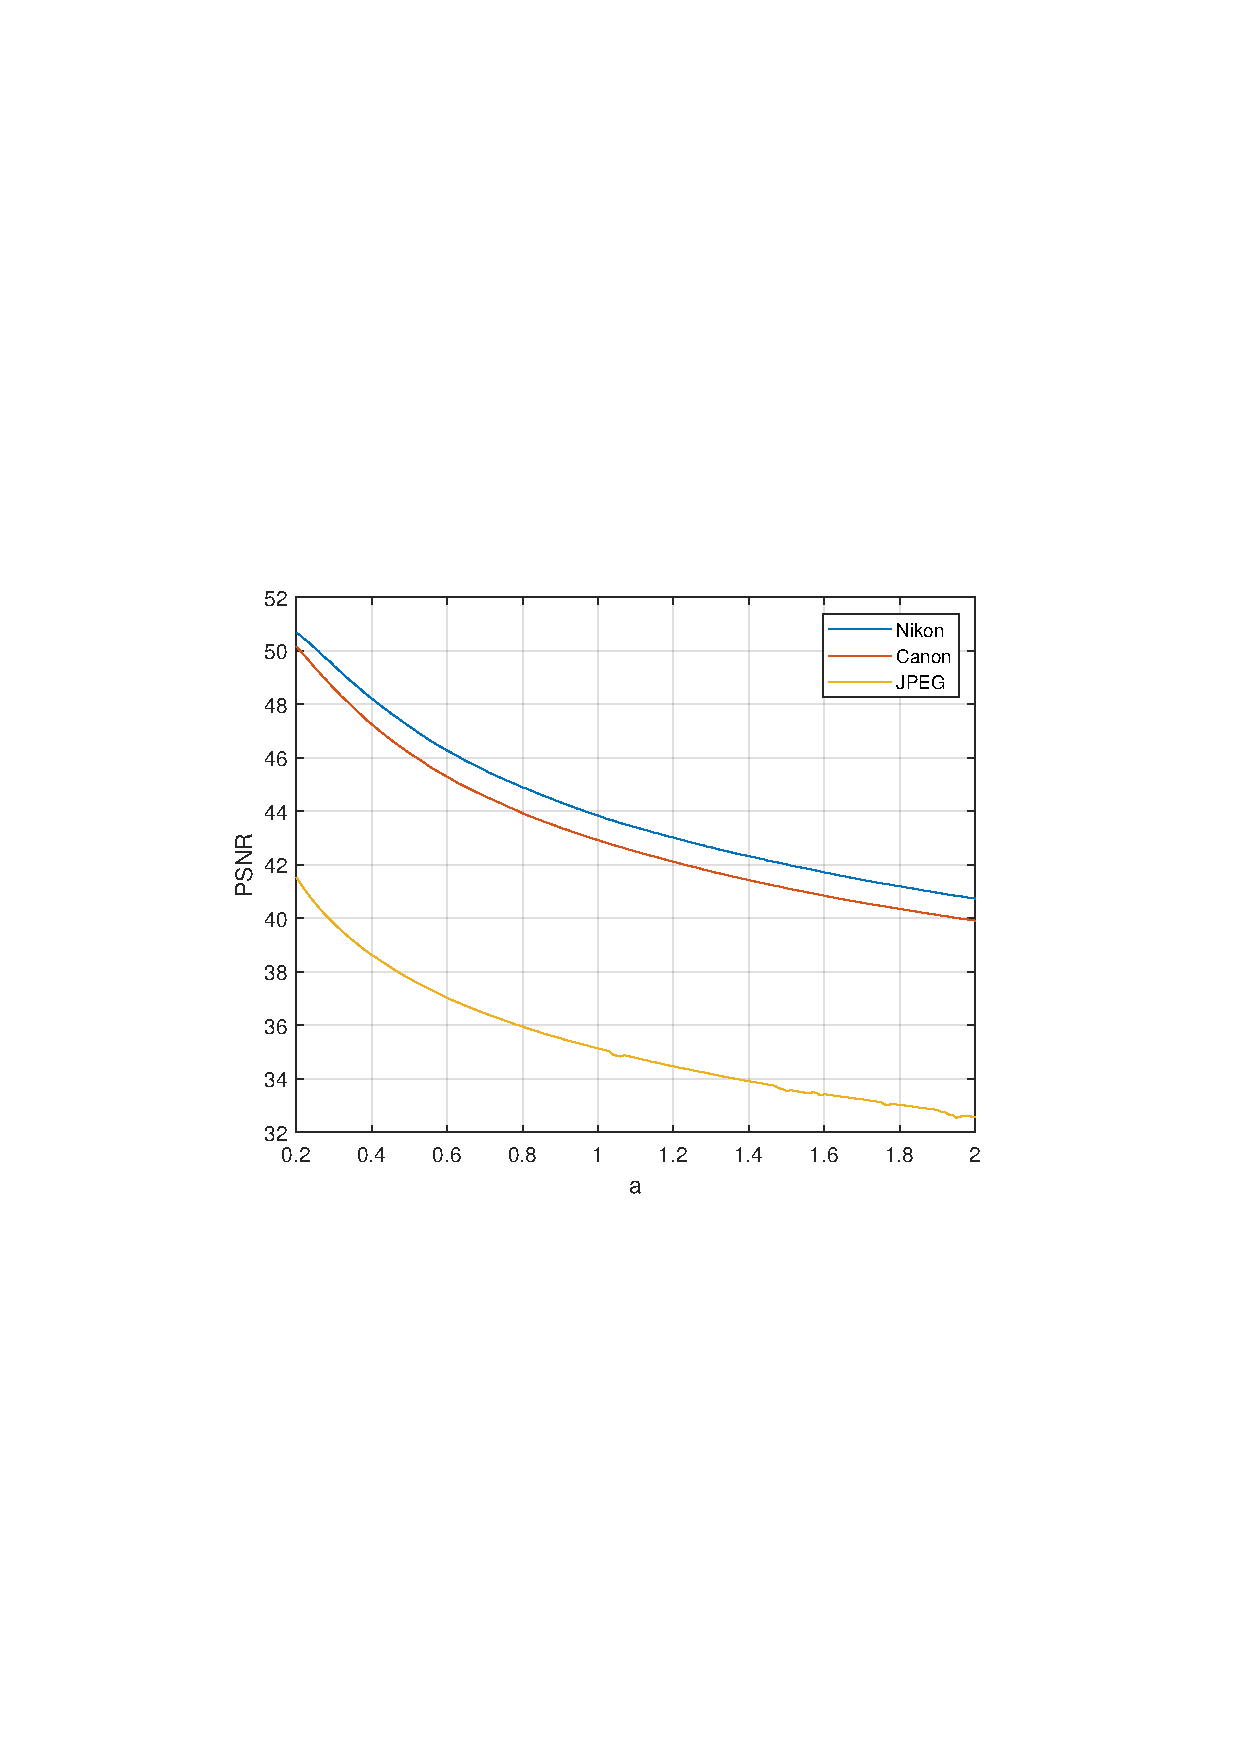
\includegraphics[width=0.8\textwidth,trim={3.09cm 9.295cm 3.09cm 9.295cm},clip]{../output/quant_factor_psnr.pdf}
    \caption{随系数$a$的变化,量化表$aQ$的PSNR}
    \label{fig:quant_factor_psnr}
\end{figure}

\begin{figure}[H]
    \centering
    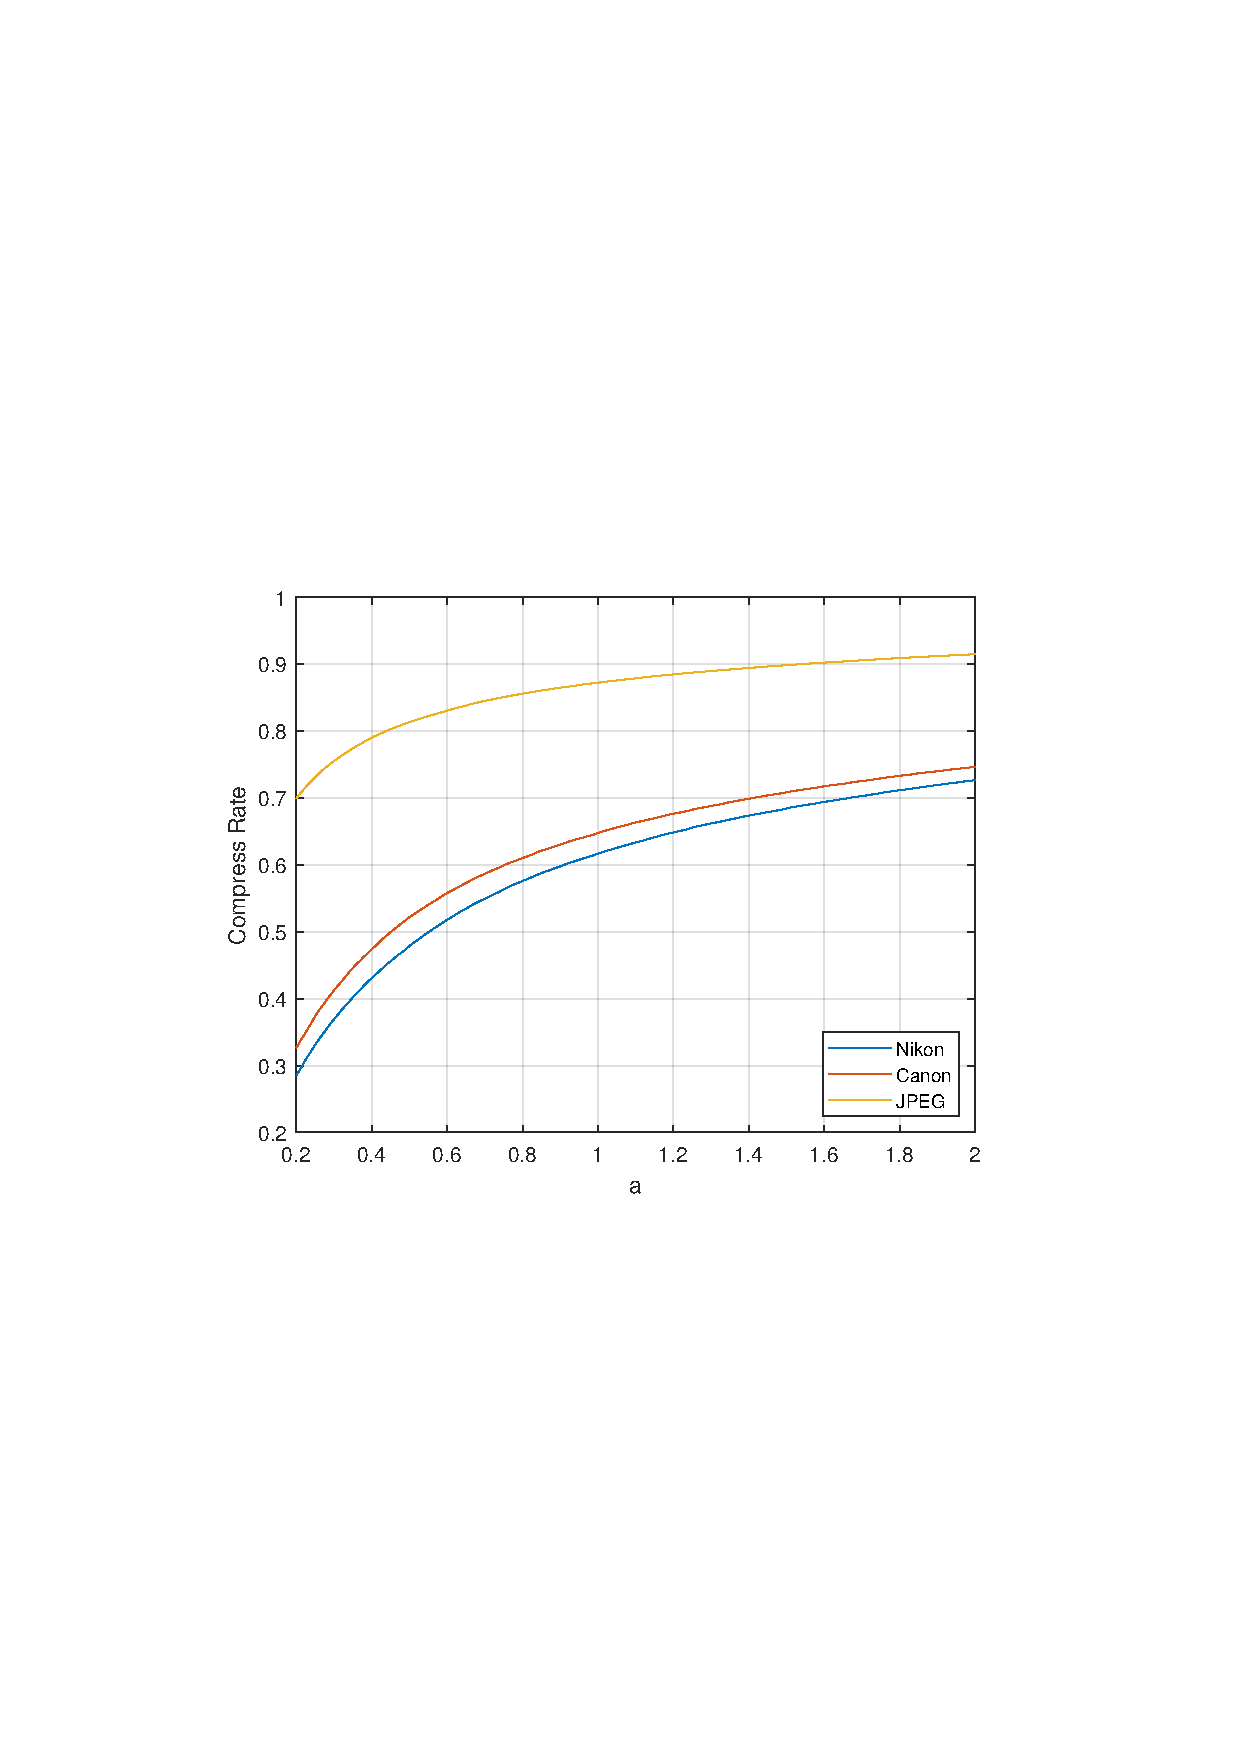
\includegraphics[width=0.8\textwidth,trim={3.09cm 9.295cm 3.09cm 9.295cm},clip]{../output/quant_factor_compress.pdf}
    \caption{随系数$a$的变化,量化表$aQ$的压缩率}
    \label{fig:quant_factor_compress}
\end{figure}

\end{document}